%Simon Krenger: Analysis
\documentclass{report}
\usepackage{amsmath}
\usepackage{amsthm}
\usepackage{amssymb}
\usepackage[utf8]{inputenc} 
\usepackage{graphicx}
\usepackage{mathtools}
\usepackage{floatrow}

\usepackage{color}
\definecolor{red}{rgb}{1,0,0}

\newtheorem{mydef}{Definition}
\newtheorem{myexample}{Beispiel}
\newtheorem{myproof}{Beweis}
\newtheorem{axiom}{Axiom}
\newtheorem{satz}{Satz}

\title{Analysis}
\author{Simon Krenger\\Gilles Bertholet}

\begin{document}
\maketitle
\chapter{Folgen und Grenzwerte}
\section{Folgengesetze}
Betrachten wir Zahlenfolgen wie
\begin{enumerate}
\item $5, 9, 13, 17, 21, ...$ \label{folgen:enum1}
\item $9, 3, 1, \frac{1}{3}, \frac{1}{9}, \frac{1}{27}, ...$ \label{folgen:enum2}
\item $\frac{1}{8}, -\frac{1}{4}, \frac{1}{2}, -1, 2, -4, ... $ \label{folgen:enum3}
\item $1, 1, 2, 3, 5, 8, 13, 21, ...$ \label{folgen:enum4}
\end{enumerate}
So fällt einerseits die Gesetzmässigkeit und andererseits ein immer vorhandenes erstes Element auf.
\begin{mydef}Eine \underline{Folge} ist eine Funktion mit $\mathbb{N}$ als Definitionsmenge\end{mydef}
Für $f: \mathbb{N} \mapsto \mathbb{R}$ mit $y = f(x)$ schreiben wir bei Folgen
\begin{equation}(a_n)_{n \in \mathbb{N}} \quad \mbox{mit} \quad a_n=a(n)\end{equation}
\begin{myexample}$a_n = 3n + 7$ ist das Gesetz für die Folge $10, 13, 16, ...$\end{myexample}
Das Gesetz einer Folge können wir so angeben, dass auf das vorangehende \underline{Folgenglied} (Element) Bezug genommen wird. So erhalten wir das \underline{rekursive Gesetz}.
\\\\
Bei (\ref{folgen:enum1}) lautet dies $a_{n+1} = a_n + 4$ \underline{und} $a_1 = 5$ und bei (\ref{folgen:enum2}) $b_{n+1}=\frac{1}{3}b_n$ und $b_1=9$.
\\\\
Wir können aber auch ein Gesetz suchen, welches $a_n$ mit Hilfe von $n$ berechnet. Das nennen wir das \underline{explizite Gesetz}.
\\\\
Die Folge (\ref{folgen:enum3}) ist eine \underline{alternierende} Folge (abwechselnd $+$ und $-$). Dann muss $(-1)^n$ oder $(-1)^{n+1}$ im expliziten Gesetz stehen.\\
Bei (\ref{folgen:enum3}) also $a_n = (-1)^{n+2} \cdot 2^{n-4}$\\
Für die Folge  (\ref{folgen:enum4}) finden wir das rekursive Gesetz
\begin{equation}a_{n+1} = a_n + a_{n-1} \quad \mbox{und} \quad a_1=1, a_2=1\end{equation}
für die \underline{Fibonacci-Folge}. Das explizite Gesetz ist schwierig zu finden.

\section{Teilsummen}
Wenn wir die Elemente einer Folge addieren, so erhalten wir die n-te Teilsumme
\begin{equation}s_n = a_1 + a_2 + a_3 + ... + a_n \quad (n \in \mathbb{N})\end{equation}
\begin{equation}s_n = \sum_{k=1}^{n} a_k \quad \mbox{("Summe $a_k$, k von 1 bis n")}\end{equation}
Wollen wir zum Beispiel
\begin{equation}1 + 2 + 3 + 4 + ... + 100\end{equation}
berechnen, so greifen wir auf die Idee von Carl Friedrich Gauss (1777 bis 1855, Göttingen) zurück.
\begin{eqnarray}s_{100} & = & (1 + 100) + (2 + 99) + ... + (50 + 51) \nonumber \\
& = & 50 \cdot 101 \nonumber \\
& = & 5050\end{eqnarray}
Wollen wir
\begin{equation}s_n = \frac{1}{2 \cdot 5} + \frac{1}{5 \cdot 8} + \frac{1}{8 \cdot 11} + ... + a_n\end{equation}
berechnen, so bestimmen wir die \underline{Teilsummenfolge}.
\begin{eqnarray}s_1 & = & \frac{1}{10}\\
s_2 & = & \frac{1}{10} + \frac{1}{5 \cdot 8} = \frac{8 + 2}{2 \cdot 5 \cdot 8} = \frac{10}{80} = \frac{1}{8} \textcolor{red}{ = \frac{2}{16}}\\
s_3 & = & \frac{1}{8} + \frac{1}{8 \cdot 11} = \frac{11 + 1}{8 \cdot 11} = \frac{12}{8 \cdot 11} = \frac{3}{22}\\
s_4 & = & \frac{3}{22} + \frac{1}{11 \cdot 14} = \frac{42 + 2}{2 \cdot 11 \cdot 14} = \frac{2}{14} = \frac{1}{7} \textcolor{red}{ = \frac{4}{28}}\end{eqnarray}
also finden wir
\begin{equation}s_n = \frac{n}{6n + 4}\end{equation}
Wir beweisen mit vollständiger Induktion.
\begin{myproof}\begin{enumerate}
\item \label{proof:teilsummenfolge-1} Behauptung ist für $n=1$ wahr, denn
\begin{equation}s_1 = \frac{1}{10}\end{equation}
und $s_n$ wird mit $n=1$ zu
\begin{equation}s_1 = \frac{1}{6 \cdot 1 + 4} = \frac{1}{10}\end{equation}
\item \label{proof:teilsummenfolge-2} Voraussetzung: 
\begin{equation}s_n = \frac{n}{6n+4}\end{equation}
Behauptung:
\begin{equation}s_{n+1} = \frac{n+1}{6(n+1) + 4} = \frac{n+1}{6n+10}\end{equation}
Beweis:
\begin{equation}s_{n+1} = s_n + a_{n+1}\end{equation}
und wir müssen $a_{n+1}$ bestimmen. Es ist
\begin{equation}a_n = \frac{1}{(3n-1)(3n+2)}\end{equation}
, also
\begin{eqnarray}a_{n+1} & = & \frac{1}{(3(n+1)-1)(3(n+1)+2)} \\
& = & \frac{1}{(3n+2)(3n+5)}\end{eqnarray}
Somit ist
\begin{eqnarray}s_{n+1} & = & \frac{n}{6n+4} + \frac{1}{(3n+2)(3n+5)} \\
& = & \frac{n}{2(3n+2)} + \frac{1}{(3n+2)(3n+5)} \\
& = & \frac{3n^2+5n+2}{2(3n+2)(3n+5)} \\
& = & \frac{(3n+2)(n+1)}{2(3n+2)(3n+5)} \\
& = & \frac{n+1}{2(3n+5)} = \frac{n+1}{6n+10}\end{eqnarray}
\item Nach (\ref{proof:teilsummenfolge-1}) ist die Behauptung für $n=1$ wahr und nach (\ref{proof:teilsummenfolge-2}) für $n+1$, also für $n=2$ usw. Also ist die Behauptung für alle $\mathbb{N}$ wahr.
\end{enumerate}\end{myproof}
Natürlich finden wir auch sofort
\begin{equation}\sum_{k=1}^{n} k = 1 + 2 + ... + n = (1+n)\frac{n}{2}\end{equation}

\section{Grenzwerte}
Zeichnen wir die Elemente von
\begin{equation}a_n = (-1)^n(2+\frac{1}{n})\end{equation}
auf der Zahlengeraden,
\\\\TODO\\\\
so häufen sich die Werte bei 2 und -2. Sowohl in der Nähe von 2 als auch -2 liegen unendlich viele Werte.
\begin{mydef}Wir nennen
\begin{equation}U_\epsilon(a) := [a-\epsilon; a + \epsilon]; \epsilon \in \mathbb{R}^+\end{equation}
eine \underline{$\epsilon$-Umgebung} von $a$.\end{mydef}
\begin{mydef}Finden wir in jeder $\epsilon$-Umgebung einer Zahl $a$ unendlich-viele Folgenglieder, so heisst $a$ ein Häufungswert der Folge $(a_n)$.\end{mydef}
\begin{myexample}\begin{enumerate}
\item \begin{eqnarray}a_n & = & \frac{n+1}{n} \nonumber \\
& \rightarrow & 2, 1.5, 1.\bar{3}, 1.25, 1.2, 1.16, 1.\bar{142857}\end{eqnarray}
also ist 1 ein Häufungswert.
\item \begin{eqnarray}b_n & = & 4n + 1 \nonumber \\
& \rightarrow & 5, 9, 13, 17, ...\end{eqnarray}
Also kein Häufungswert.\end{enumerate}\end{myexample}
Besitzt eine Folge genau einen einzigen Häufungswert, so nennen wir diesen den \underline{Limes} (Grenzwert) der Folge und schreiben
\begin{equation}\lim_{n \to \infty}a_n = a \end{equation}
\begin{myexample}\begin{enumerate}
\item \begin{equation}\lim_{n \to \infty}\frac{n+1}{n}=1\end{equation}
\item \begin{equation}\lim_{n \to \infty}(-1)^n(2+\frac{1}{n})\end{equation}
\item \begin{equation}\lim_{n \to \infty}\frac{1}{n}=0\end{equation}
\end{enumerate}\end{myexample}
\begin{mydef}Im Folgenden die Definition des Limes nach Cauchy (Louis Augustin Cauchy, 1789 bis 1857, Paris, Schweiz, Prag):\\
Eine Zahlenfolge $(a_n)$ besitzt den Grenzwert $a$, wenn für alle $\epsilon > 0$ von einem bestimmten $n$ an, alle weiteren Folgenglieder in $U_\epsilon(a)$ liegen:
\begin{equation}\epsilon \in \mathbb{R}, n_0 \in \mathbb{N}: \forall \epsilon > 0\exists n_0 \forall n (n > n_0 \to |a_n-a| < \epsilon)\end{equation}\end{mydef}
\begin{myexample}$a_n = \frac{5}{n}$ hat Grenzwert $a=0$\\
Ist $\epsilon = \frac{1}{100}$, so wird $n_0 = 500$, denn von $a_{501}$ an sind alle Folgenglieder zwischen $0,01$ und $0$.\end{myexample}
\begin{mydef}Besitzt eine Folge einen Grenzwert, so heisst sie \underline{konvergent}, andernfalls \underline{divergent}. Folgen mit Grenzwert $0$ heissen \underline{Nullfolgen}.\end{mydef}
\begin{myexample}Wir untersuchen diese Folgen:\begin{enumerate}
\item \begin{equation}\lim_{n \to \infty}\frac{1}{n}=0, \lim_{n \to \infty}\frac{k}{n} = 0, k \in \mathbb{Z} \setminus \{0\}\end{equation}
\item \begin{equation}\lim_{n \to \infty}\frac{1}{n^2}=0, \lim_{n \to \infty}\frac{k}{n^2} = 0, k \in \mathbb{Z} \setminus \{0\}\end{equation}
\item \begin{equation}\lim_{n \to \infty}\frac{1}{n^k}=0, k \in \mathbb{N}\end{equation}
\item \begin{equation}\lim_{n \to \infty}2^n\end{equation} existiert nicht, die Folge $a_n = 2^n$ \underline{wächst über alle Schranken}; sie ist also divergent.
\item \begin{equation}\lim_{n \to \infty}(2+\frac{1}{n}) = \lim_{n \to \infty}2 + \lim_{n \to \infty}\frac{1}{n} = 2\end{equation}
\item \begin{equation}\lim_{n \to \infty}\frac{3n^2+5}{n^2} = \lim_{n \to \infty}3 + \lim_{n \to \infty}\frac{5}{n^2} = 3\end{equation}
\item \begin{equation}\lim_{n \to \infty}\frac{4n-7}{3n+1} \neq \frac{\lim_{n \to \infty}4n-7}{\lim_{n \to \infty}3n+1}\end{equation}
\end{enumerate}\end{myexample}
\newpage
Wir brauchen die \underline{Grenzwertsätze}. Sind $(a_n)$ und $(b_n)$ konvergent mit $\lim_{n \to \infty}a_n = a, \lim_{n \to \infty}b_n = b$, so ist
\begin{enumerate}
\item \begin{equation}\lim_{n \to \infty}(a_n + b_n) = \lim_{n \to \infty}a_n + \lim_{n \to \infty}b_n = a + b\end{equation}
\item \begin{equation}\lim_{n \to \infty}(a_n \cdot b_n) = \lim_{n \to \infty}a_n \cdot \lim_{n \to \infty}b_n = a \cdot b\end{equation}
\item \begin{equation}\forall n (b_n \neq 0) \land b_n \neq 0 :\\
\lim_{n \to \infty}\frac{a_n}{b_n} = \frac{\lim_{n \to \infty}a_n}{\lim_{n \to \infty}b_n} = \frac{a}{b}\end{equation}
\end{enumerate}
Um
\begin{equation}\lim_{n \to \infty}\frac{5n-2}{6n+1}\end{equation}
zu berechnen, überlegen wir, dass Brüche gekürzt werden können und kürzen mit n.
\begin{eqnarray}\lim_{n \to \infty}\frac{5n-2}{6n+1} & = & \lim_{n \to \infty}\frac{\frac{5n-2}{n}}{\frac{6n+1}{n}} = \lim_{n \to \infty}\frac{\frac{5n}{n}-\frac{2}{n}}{\frac{6n}{n}+\frac{1}{n}} \nonumber \\
= \lim_{n \to \infty}\frac{5-\frac{2}{n}}{6+\frac{1}{n}} & =  &\frac{\lim_{n \to \infty}(5-\frac{2}{n})}{\lim_{n \to \infty}(6+\frac{1}{n})} = \frac{5}{6}\end{eqnarray}
\begin{myexample}Wir kürzen jeweils mit der Variabel ($n$) mit der höchsten Potenz:\begin{enumerate}
\item \begin{eqnarray}\lim_{n \to \infty}\frac{2n^2+1}{4n^2-3} & = & \lim_{n \to \infty}\frac{\frac{2n^2}{n^2}+\frac{1}{n^2}}{\frac{4n^2}{n^2}-\frac{3}{n^2}} \nonumber \\ 
= \lim_{n \to \infty}\frac{2+\frac{1}{n^2}}{4-\frac{3}{n^2}} & = & \frac{\lim_{n \to \infty}(2+\frac{1}{n^2})}{\lim_{n \to \infty}(4-\frac{3}{n^2})} = \frac{2}{4} = \frac{1}{2}\end{eqnarray}
\item \begin{equation}\lim_{n \to \infty}\frac{n^2+2n+5}{n-7} = \lim_{n \to \infty}\frac{1+\frac{2}{n} + \frac{5}{n^2}}{\frac{1}{n} - \frac{7}{n^2}}\end{equation}
existiert nicht.
\item \begin{eqnarray}\lim_{n \to \infty}\frac{\sqrt{n}+\sqrt{n-1}}{\sqrt{n}-\sqrt{2n-1}} & = & \lim_{n \to \infty}\frac{\frac{\sqrt{n}}{\sqrt{n}}+\frac{\sqrt{n-1}}{\sqrt{n}}}{\frac{\sqrt{n}}{\sqrt{n}}-\frac{\sqrt{2n-1}}{\sqrt{n}}} = \lim_{n \to \infty}\frac{1+\frac{\sqrt{n-1}}{\sqrt{n}}}{1-\frac{\sqrt{2n-1}}{\sqrt{n}}} \nonumber \\
= \lim_{n \to \infty}\frac{1+\sqrt{1-\frac{1}{n}}}{1-\sqrt{2-\frac{1}{n}}} &=& \frac{1+\sqrt{1}}{1-\sqrt{2}} = \frac{2}{1-\sqrt{2}}\end{eqnarray}
\end{enumerate}\end{myexample}
\newpage
Um
\begin{equation}\lim_{n \to \infty} (1+\frac{1}{n})^n\end{equation}
zu berechnen, bestimmen wir
\\\\$a_{100} = 2,70481...$, $a_{1000} = 2,7169...$\\\\
und finden, dass die Folge beschränkt ist. Es ist
\begin{equation}\lim_{n \to \infty} (1 + \frac{1}{n})^1 = e\end{equation}
und $e = 2,71828...$ ist irrational und transzendent.
\begin{myexample}Wir betrachten\begin{enumerate}
\item \begin{equation}\lim_{n \to \infty} ( 1 + \frac{1}{5n})^{5n} = e\end{equation}
\item \begin{equation}\lim_{n \to \infty} ( 1 + \frac{1}{\frac{n}{3}})^{\frac{n}{3}} = e\end{equation}
\item \begin{equation}\lim_{n \to \infty} ( 1 + \frac{1}{n})^{4n} = \lim_{n \to \infty}[ ( 1 + \frac{1}{n})^{n}]^4 = e^4\end{equation}
\end{enumerate}\end{myexample}
Wollen wir
\begin{equation}\lim_{n \to \infty} ( 1 + \frac{k}{n})^n, k \in \mathbb{Z}\end{equation}
berechnen, so überlegen wir, dass
\begin{equation}1 + \frac{k}{n} ) 1 + \frac{1}{\frac{n}{k}}\end{equation}
und finden
\begin{equation}\lim_{n \to \infty} ( 1 + \frac{1}{\frac{n}{k}})^\frac{n}{k} = e\end{equation}
Weiter ist dann
\begin{equation}\lim_{n \to \infty} (1 + \frac{k}{n})^n = \lim_{n \to \infty}[(1 + \frac{k}{\frac{n}{k}})^\frac{n}{k}]^k = e^k\end{equation}
und damit
\begin{equation}\lim_{n \to \infty} (1 - \frac{1}{n})^n = \lim_{n \to \infty} (1 + \frac{-1}{n})^n = e^{-1}\end{equation}
Zusammengefasst
\begin{eqnarray}\lim_{n \to \infty} (1 + \frac{1}{n})^n & = & e\\
\lim_{n \to \infty} (1 - \frac{1}{n})^n & = & \frac{1}{e} = e^{-1}\\
\lim_{n \to \infty} (1 + \frac{k}{n})^n & = & e^k, k \in \mathbb{Z}\end{eqnarray}

\section{Reihen}
\begin{mydef}Ist $(a_n)$ eine Folge, so heisst
\begin{equation}\sum_{n=1}^{\infty}a_n = a_1 + a_2 + a_3 + ...\end{equation}
eine \underline{Reihe}.\end{mydef}
Wollen wir
\begin{equation}\sum_{n=1}^{\infty}\frac{1}{n (n+1)} = \frac{1}{1 \cdot 2} + \frac{1}{2 \cdot 3} + \frac{1}{3 \cdot 4} + ...\end{equation}
bestimmen, so nützen wir
\begin{equation}\frac{1}{n(n+1)} = \frac{1}{n}-\frac{1}{n+1}\end{equation}
aus und erhalten so
\begin{eqnarray}\sum_{n=1}^{\infty} \frac{1}{n (n+1)} & = & \sum_{n=1}^{\infty} \frac{1}{n}-\frac{1}{n+1}\nonumber \\
& = & 1 - \frac{1}{2} + \frac{1}{2} - \frac{1}{3} + \frac{1}{3} - \frac{1}{4} + ... = 1\end{eqnarray}
Um die Reihe
\begin{equation}\sum_{n=1}^{\infty} \frac{1}{(3n-1)(3n+2)}\end{equation}
zu berechnen, bestimmen wir die \underline{Teilsummenfolge (Partialsummenfolge)}
\\\\$s_1, s_2, s_3, ...$\\\\
und überlegen dann, ob diese Folge einen Grenzwert besitzt.
\begin{eqnarray}s_n & = & \sum_{k=1}^{\infty} \frac{1}{(3k-1)(3k+2)} \nonumber \\
&=& \frac{1}{2 \cdot 5} + \frac{1}{5 \cdot 8} + \frac{1}{8 \cdot 11} + ... + a_n\end{eqnarray}
und so
\begin{eqnarray}s_1 & = & \frac{1}{10} \nonumber \\
s_2 & = & \frac{1}{10} + \frac{1}{5 \cdot 8} = \frac{8+2}{2 \cdot 5 \cdot 8} = \frac{10}{80} = \frac{1}{8} (= \frac{2}{16}) \nonumber \\
s_3 & = & \frac{1}{8} + \frac{1}{8 \cdot 11} = \frac{12}{8 \cdot 11} = \frac{3}{22}\end{eqnarray}
, also
\begin{equation}s_n = \frac{n}{6n+4}\end{equation}
und so
\begin{equation}\sum_{n=1}^{\infty} \frac{1}{(3n-1)(3n+2)} = \lim_{n \to \infty} \frac{n}{6n+4} = \frac{1}{6}\end{equation}
Wir sagen dann, dass die Reihe konvergent ist und der \underline{Wert der Reihe} ist $\frac{1}{6}$.
\begin{mydef}Wir nennen
\begin{equation}\sum_{n=1}^{\infty} a_1 q^{n-1} = a_1 + a_1 q + a_1 q^2 + ... \quad \mbox{mit} \quad q \neq 0,1\end{equation}
eine \underline{geometrische Reihe}.\end{mydef}
\begin{myexample}\begin{enumerate}
\item \begin{equation}\sum_{n=1}^{\infty} 2^{n-3} = \frac{1}{4} + \frac{1}{2} + 1 + 2 + 4 + ...\end{equation}
\item \begin{equation}\sum_{n=1}^{\infty} 4(\frac{1}{3})^{n-1} = 4 + \frac{4}{3} + \frac{4}{9} + \frac{4}{27} + ...\end{equation}
\end{enumerate}\end{myexample}
Es ist also der \underline{Quotient} $q \neq 0,1$ zweier aufeinanderfolgenden Glieder stets gleich. Um Den Wert der Reihe zu bestimmen, betrachten wir
\begin{eqnarray}s_n & = & a_1 + a_1 \cdot q + a_1 \cdot q^2 + ... + a_1 \cdot q^{n-1} \nonumber \\
- ( q \cdot s_n & = & a_1 \cdot q + a_1 \cdot q^2 + a_1 \cdot q^3 + ... + a_1 \cdot q^n ) \nonumber \\\\
s_n - q \cdot s_n & = & a_1 - a_1 \cdot q^n \nonumber \\
s_n (1-q) & = &  a_1(1-q^n)\end{eqnarray}
Damit
\begin{equation}s_n = \frac{a_1(1-q^n)}{(1-q)} \quad \mbox{mit} \quad q \neq 0,1\end{equation}
Dann ist
\begin{equation}\sum_{n=1}^{\infty} a_1 q^{n-1} = \lim_{n \to \infty} \frac{a_1(1-q^n)}{(1-q)}\end{equation}
und für $q > 1 \lor q < -1$ existiert der Grenzwert nicht. Für $-1 < q < 1$ ist
\begin{equation}\lim_{n \to \infty}\frac{a_1(1-q^n)}{1-q} = \frac{a_1}{1-q} \quad \mbox{, da} \quad \lim_{n \to \infty}q^n = 0\end{equation}
Also ist der Wert der geometrischen Reihe
\begin{equation}\sum_{n=1}^{\infty}a_1q^{n-1} = \frac{a_1}{1-q} \quad \mbox{mit} \quad -1 < q < 1\end{equation}
\begin{myexample}\begin{equation}2 - 1 + \frac{1}{2} - \frac{1}{4} + \frac{1}{8} - ... = \frac{2}{1-(-\frac{1}{2})} = \frac{4}{3}\end{equation}\end{myexample}
\begin{mydef}Wir nennen
\begin{equation}s = 1 + \frac{1}{2} + \frac{1}{3} + \frac{1}{4} + ...\end{equation}
die \underline{harmonische Reihe}.\end{mydef}
$s$ ist nicht konvergent, denn es ist
\begin{equation}1 + \frac{1}{2} = \frac{3}{2}\end{equation}
und
\begin{equation}\frac{1}{3} + \frac{1}{4} = \frac{7}{12} \textcolor{red}{ = 0,5837... > \frac{1}{2}}\end{equation}
und
\begin{equation}\frac{1}{5} + \frac{1}{6} + \frac{1}{7} + \frac{1}{8} = \frac{533}{840} \textcolor{red}{ = 0.634... > \frac{1}{2}}\end{equation}
also
\begin{equation}s = 1 + \frac{1}{2} + \frac{1}{3} +\frac{1}{4} +\frac{1}{5} +\frac{1}{6} +\frac{1}{7} +\frac{1}{8} +\frac{1}{9} + ...\end{equation}
So ist $s$ divergent! Hingegen ist
\begin{equation}1 + \frac{1}{2!} +\frac{1}{3!} +\frac{1}{4!} + ... = \sum_{k=0}^{\infty} \frac{1}{k!} = e\end{equation}
und
\begin{equation}1 + \frac{1}{2^2} +\frac{1}{3^2} +\frac{1}{4^2} + ... = \frac{\pi^2}{6}\end{equation}
und die \underline{Leibnizsche Reihe}
\begin{equation}1 - \frac{1}{3} +\frac{1}{5} -\frac{1}{7} + \frac{1}{9} - ... = \frac{\pi}{4}\end{equation}

\section{Stetigkeit}
Wir wollen für eine Funktion
\begin{equation}f: D_f \mapsto \mathbb{R}\end{equation}
den Grenzwert
\begin{equation}\lim_{x \to a} f(x)\end{equation}
bestimmen. Dazu brauchen wir eine Folge
\begin{equation}x_1, x_2, x_3, ...\end{equation}
mit Grenzwert $a$.
\\\\TODO: Graph\\\\
Nun bestimmen wir die Folge
\begin{equation}f(x_1), f(x_2), f(x_3), ...\end{equation}
und suchen deren Limes.
\\\\TODO: Graph\\\\
Bei der Funktion $g$ mit einer \underline{Sprungstelle bei $a$} hat
\begin{equation}g(x_1), g(x_2), ...\end{equation}
den Limes $b$. Aber
\begin{equation}g({x_1}'), g({x_2}'), ...\end{equation}
hat den Limes $c$. Also existiert
\begin{equation}\lim_{x \to a} g(x)\end{equation}
nicht. Beide Reihen $(x_1, x_2, x_3, ...)$ $({x_1}', {x_2}', {x_3}')$ müssen den gleichen Grenzwert besitzen.\\
Um
\begin{equation}\lim_{x \to a} f(x)\end{equation}
zu bestimmen, müssen \underline{alle} Folgen von x-Werten mit Grenzwert $a$ betrachtet werden. Wenn die Folgen der zugehörigen Funktionswerte alle denselben Limes besitzen, so ist dies $\lim_{x \to a} f(x)$.
\begin{myexample}\begin{enumerate}
\item \begin{equation}\lim_{x \to 1} x^2-2\end{equation}
\begin{center}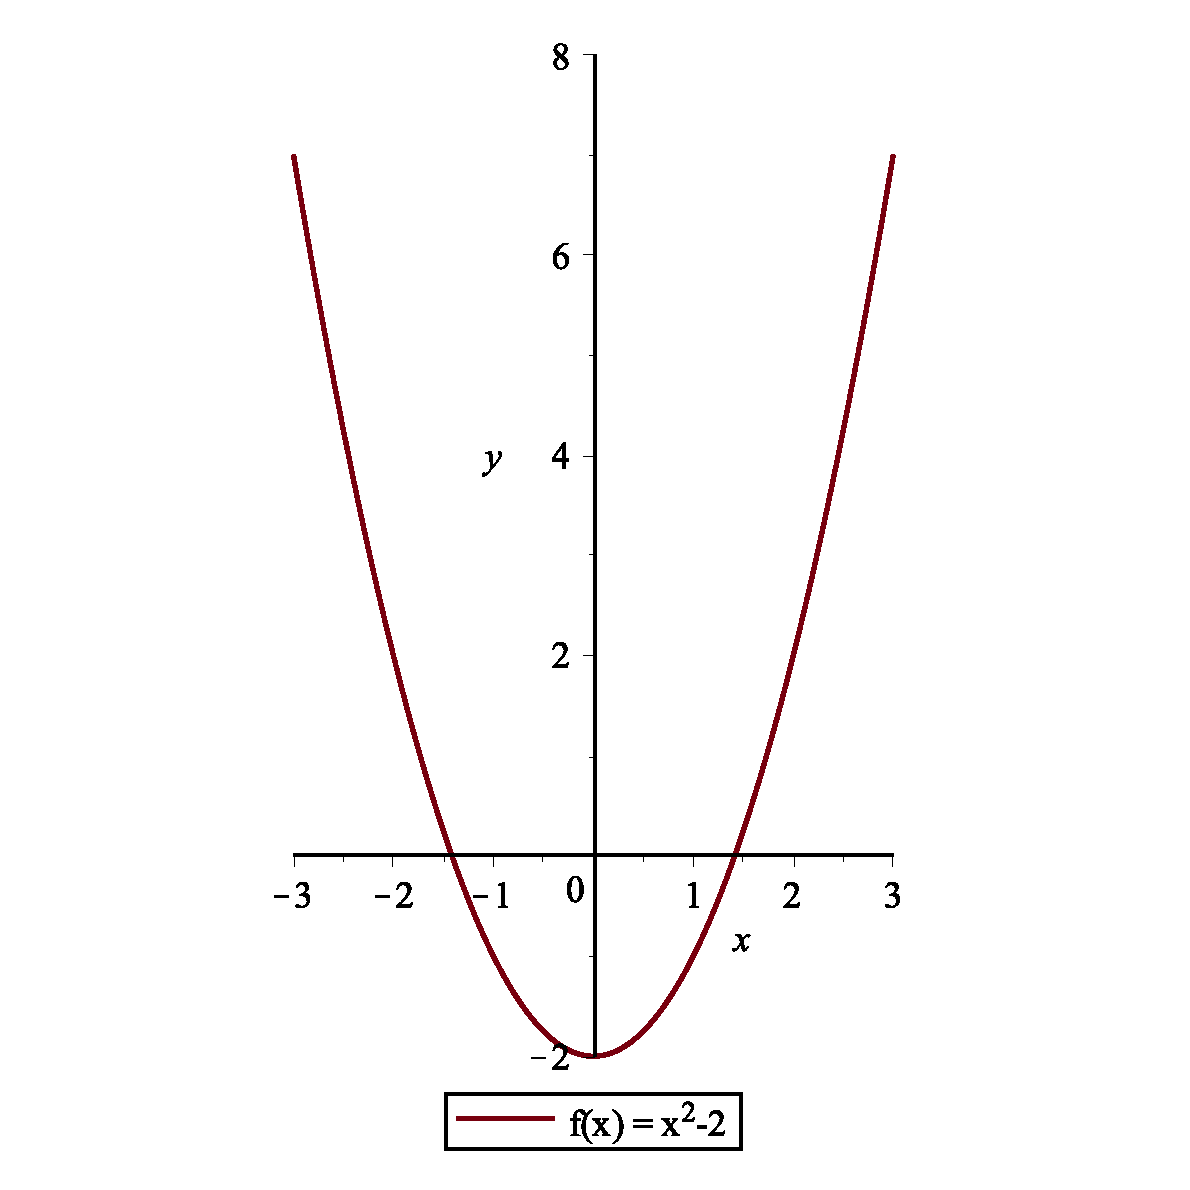
\includegraphics[scale=0.2]{images/limes_x2-2.eps}\end{center}
\begin{equation}\lim_{x \to 1} x^2-2 = 1^2 -2 = -1\end{equation}
\item \begin{equation}\lim_{x \to 3} \frac{1}{x-3}\end{equation}
\begin{center}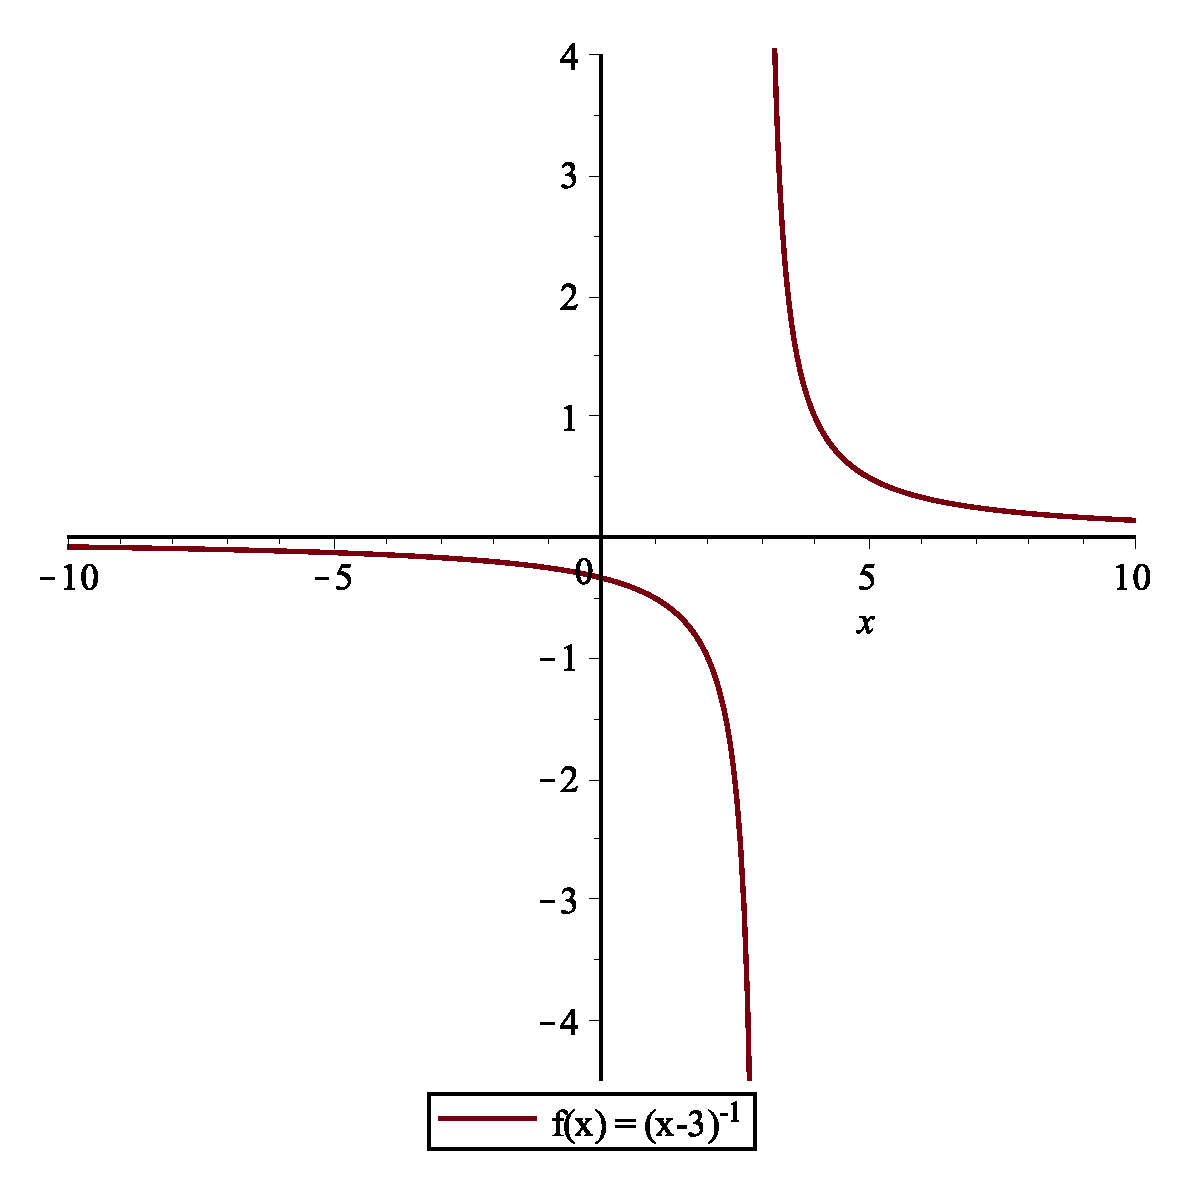
\includegraphics[scale=0.2]{images/limes_x-3.eps}\end{center}
$g(x) = \frac{1}{x-3}$ besitzt einen \underline{Pol bei $x = 3$}, also existiert $\lim_{x \to 3} \frac{1}{x-3}$ nicht.
\item \begin{equation}\lim_{x \to 0} sgn(x) \quad \mbox{("Signum von x")}\end{equation}Es ist
\[
 sgn(x) := \begin{dcases*}
        -1  &, falls $x < 0$\\
        0 &, falls $x = 0$\\
	1 & , falls $x > 0$
        \end{dcases*}
\]
\begin{center}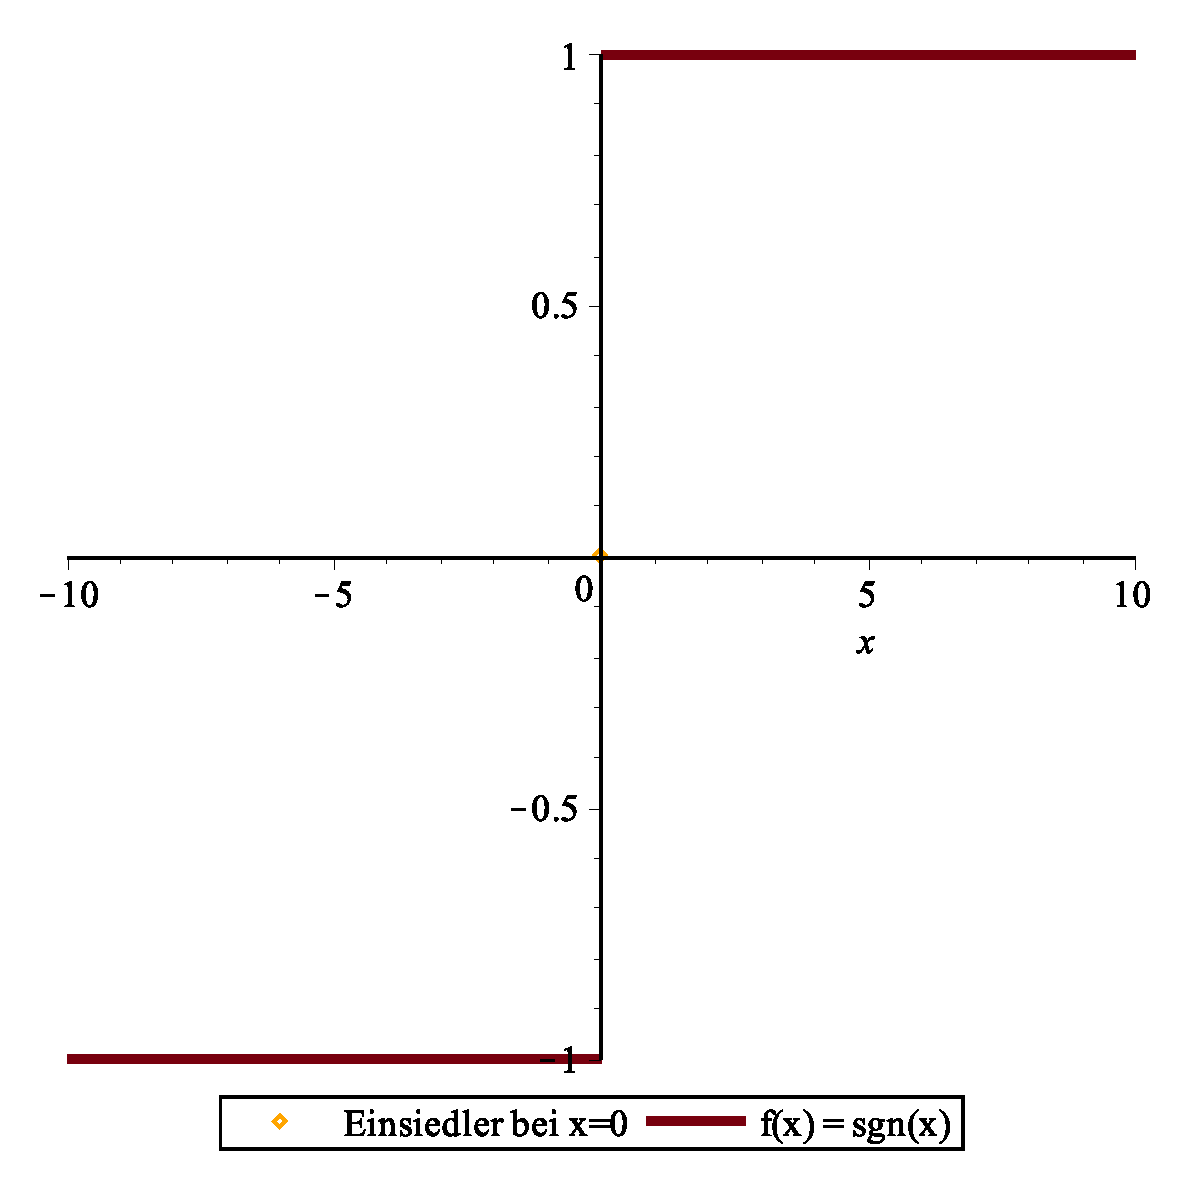
\includegraphics[scale=0.2]{images/limes_sgn_x.eps}\end{center}
$f: \mathbb{R} \mapsto \{ -1, 0, 1\}$ mit $f(x) = sgn(x)$ besitzt für $x=0$ einen \underline{isolierten Punkt (Einsiedler)}. Also existiert $\lim_{x \to 0} sgn(x)$ nicht.
\item \begin{equation}f(x) = [x] \quad \mbox{("Gausssche Klammer")}\end{equation}
\begin{center}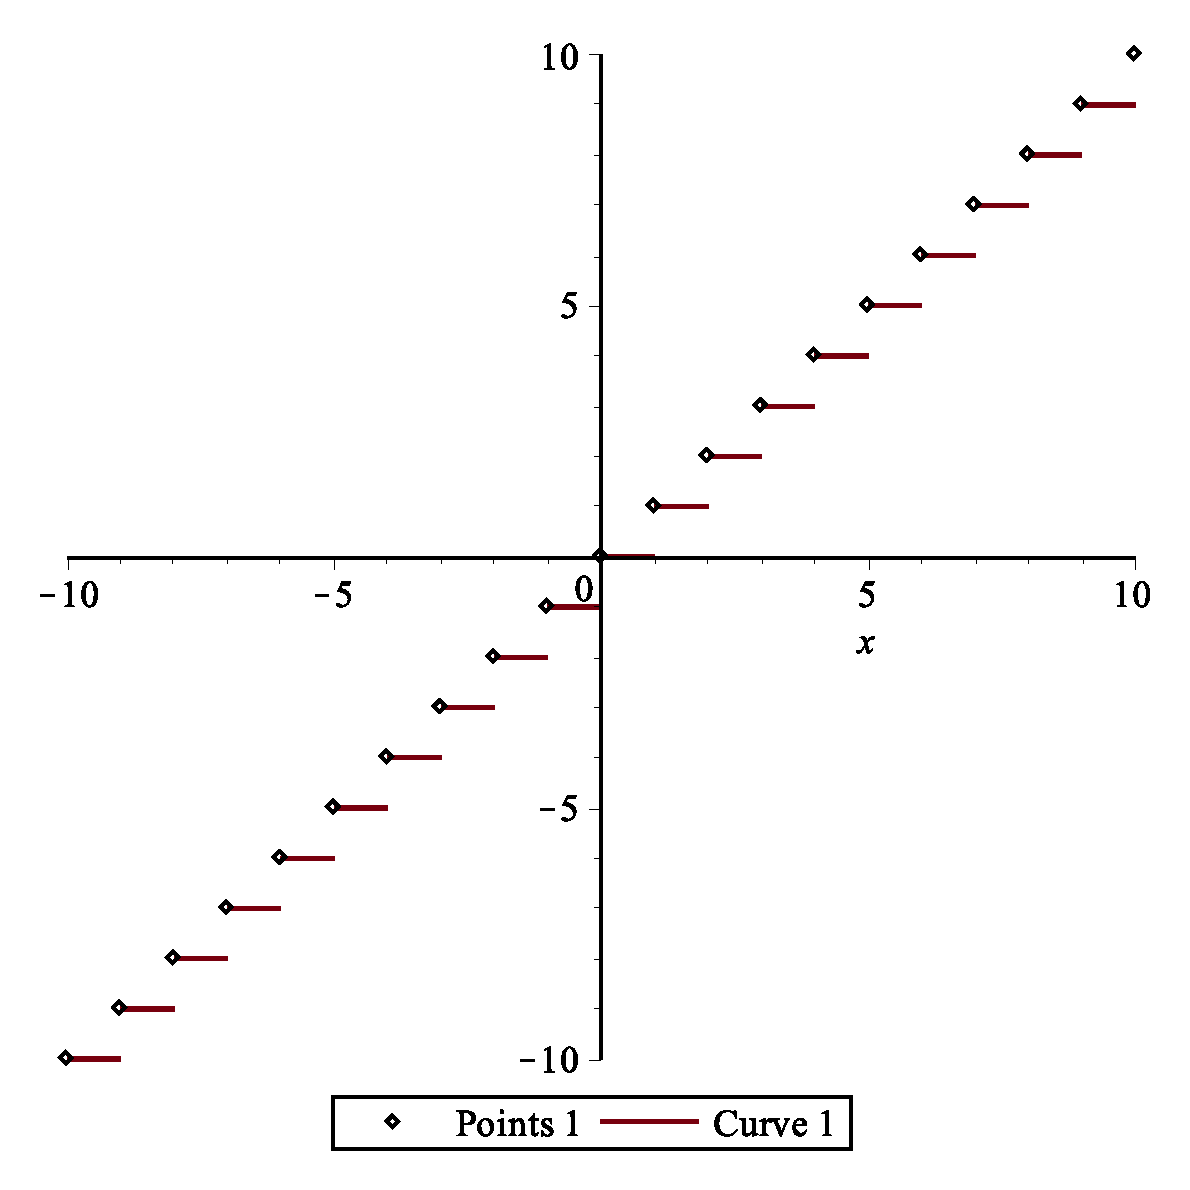
\includegraphics[scale=0.2]{images/limes_floor_x.eps}\end{center}
\end{enumerate}\end{myexample}
Besitzt eine Funktion weder isolierte Punkte noch Sprungstellen, so ist sie \underline{stetig}.
\begin{mydef}Eine Funktion $f: D_f \mapsto \mathbb{R}$ heisst \underline{stetig} an der Stelle $a \in D_f$, wenn
\begin{equation}\lim_{x \to a} f(x) = f(a)\end{equation}
\end{mydef}
\begin{myexample}
\begin{enumerate}
\item \begin{equation}f(x) = x^3\end{equation}
\begin{center}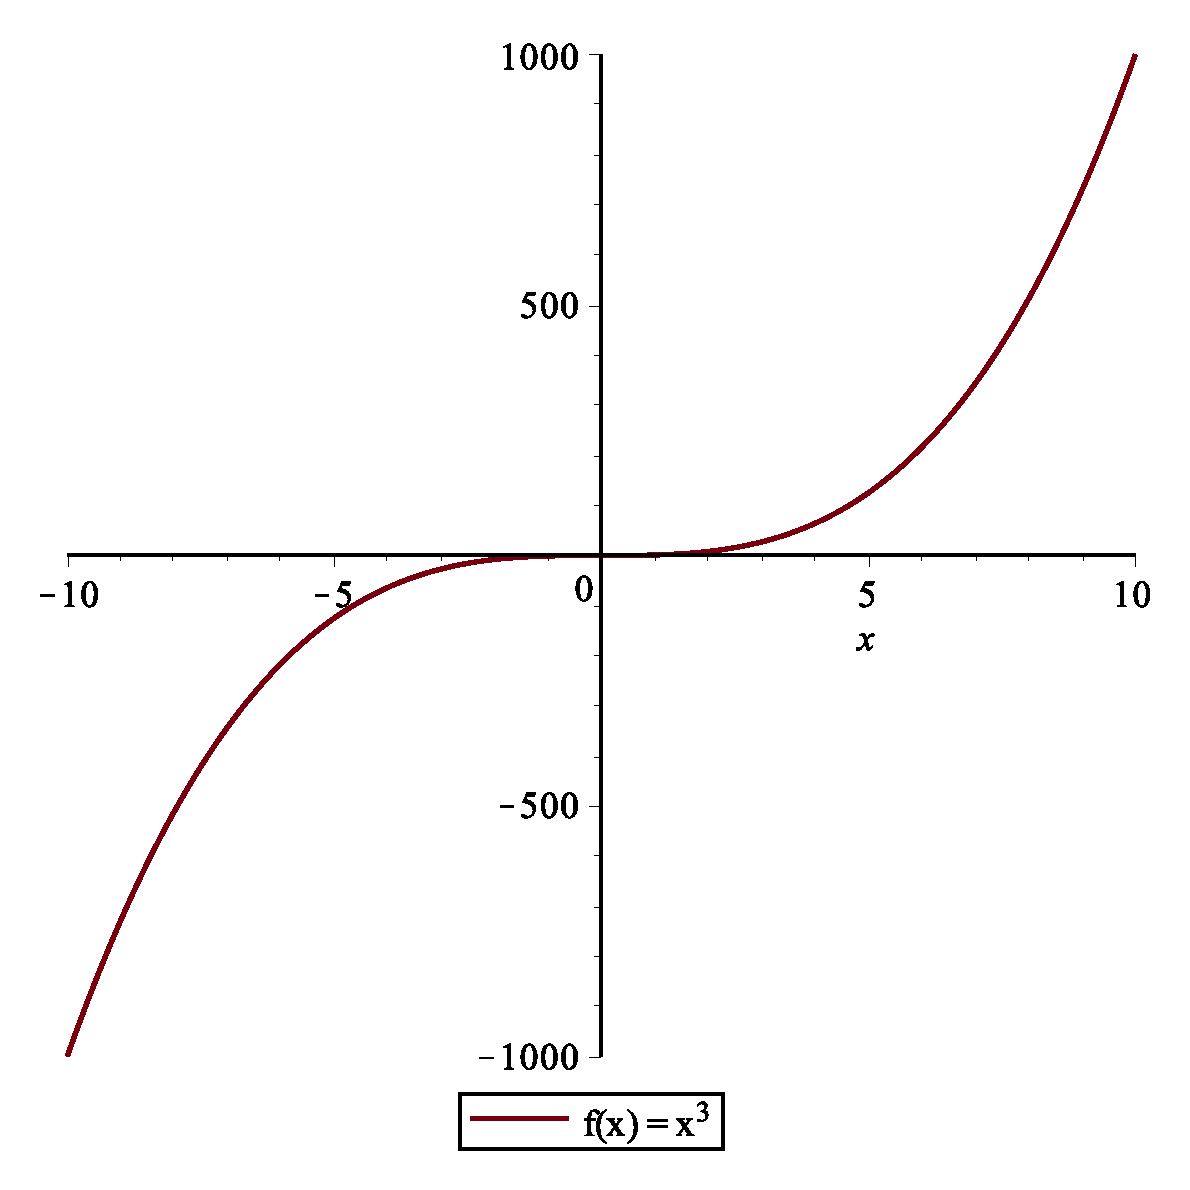
\includegraphics[scale=0.2]{images/limes_x3.eps}\end{center}
$f$ ist überall stetig.
\item \begin{equation}g: \mathbb{R} \setminus \{2\} \mapsto \mathbb{R} \quad \mbox{mit} \quad g(x) = \frac{1}{x+2}\end{equation}
\begin{center}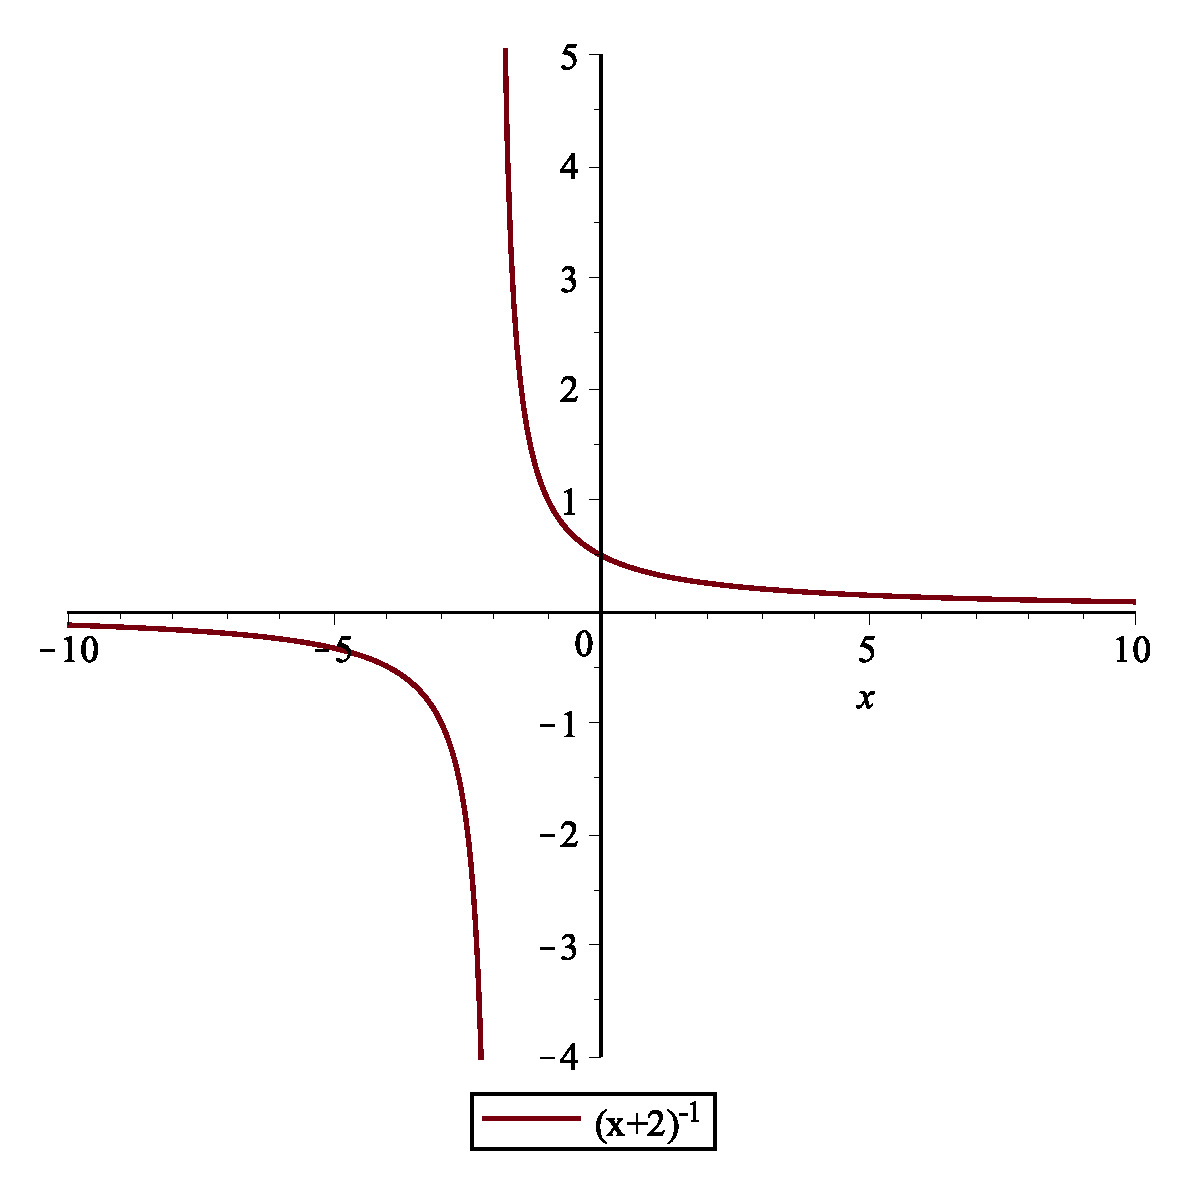
\includegraphics[scale=0.2]{images/limes_1_x-2.eps}\end{center}
$g$ ist überall stetig, denn die Stetigkeit kann nur für Werte aus der Definitionsmenge untersucht werden! Zitat Müller: "Man muss den Funktionswert berechnen können. Kann man das, so ist die Funktion stetig".
\end{enumerate}
\end{myexample}

\chapter{Differentialrechnung}
\section{Differentialquotient}
Wir betrachten eine stetige Funktion
\begin{equation}f: D_f \mapsto \mathbb{R}\end{equation}
und suchen die Steigung der Tangente an dem Graphen an der Stelle $x_0 \in D_f$.
\\\\TODO\\\\
Die Tangente ist eine spezielle Lage der Sekante. Die Steigung der Sekante ist
\begin{equation}m_s = \frac{\Delta y}{\Delta x} = \frac{f(x_0 + h) - f(x_0)}{h}\end{equation}
, was wir den \underline{Differentialquotienten} nennen. Wird $h$ immer kleiner, so nähert sich die Sekante der Tangente. Also ist die Tangentensteigung
\begin{equation}m_t = \lim_{n \to 0} \frac{f(x_0 + h) - f(x_0)}{h}\end{equation}
\begin{mydef}Wir nennen
\begin{equation}\frac{\mathrm{d}y}{\mathrm{d}x} := \lim_{n \to 0} \frac{f(x_0 + h) - f(x_0)}{h} \quad \mbox{("dy nach dx")}\end{equation}
den \underline{Differentialquotienten}.\end{mydef}
\begin{myexample}\begin{enumerate}
\item $ f:\mathbb{R} \mapsto \mathbb{R}$ mit $f(x) = x^2$ und $x_0 = 2$

Mit \begin{equation} f(x_0) = f(2) = 4 \\ f(x_0 + h) = f(2 + h) = (2+h)^2 \end{equation}
wird \begin{eqnarray} \frac{\mathrm{d}y}{\mathrm{d}x} & := & \lim_{h \to 0} \frac{(2+h)^2 - 4}{h} \\
 & := & \lim_{h \to 0}  \frac{4 + 4h + h^2 - 4}{h} \\
 & := & \lim_{h \to 0}  \frac{4h + h^2}{h} \\
 & := & \lim_{h \to 0} 4 + h \\
 & := & \underline{4} \end{eqnarray}
\item $ g:\mathbb{R} \setminus \{0\} \mapsto \mathbb{R}$ mit $g(x) = \frac{1}{x}$ und $x_0 = -3$

Mit \begin{equation} g(x_0) = g(-3) = -\frac{1}{3} \end{equation}
und \begin{equation} g(x_0 + h) = g(-3 + h) = \frac{1}{h-3} \end{equation}
\begin{eqnarray}
 \frac{\mathrm{d}y}{\mathrm{d}x} & = & \lim_{h \to 0} \frac{\frac{1}{h-3} - (-\frac{1}{3})}{h} \\
 & = & \lim_{h \to 0} \frac{\frac{1}{h-3} +\frac{1}{3}}{h} \\
 & = & \lim_{h \to 0}  \frac{\frac{3 + h-3}{3(h-3)}}{\frac{h}{1}} \\
 & = & \lim_{h \to 0} \frac{3+h-3}{3h(h-3)} \\
 & = & \lim_{h \to 0} \frac{h}{3h(h-3)} \\
 & = & \lim_{h \to 0} \frac{1}{3(h-3)} \\
 & = & \underline{-\frac{1}{9}} \end{eqnarray}
\item Gleichung der Tangente in $x_0 = 1$, wenn $ f:\mathbb{R} \mapsto \mathbb{R}$ mit $ f(x) = x^3$

Steigung mit \begin{equation} f(x_0) = f(1) = 1 \end{equation}
und \begin{equation} f(x_0 + h) = f(1 + h) = (1 + h)^3 = h^3 + 3h^2 + 3h + 1\end{equation}
\begin{eqnarray}
 \frac{\mathrm{d}y}{\mathrm{d}x} & = & \lim_{h \to 0} \frac{h^3 + 3h^2 + 3h + 1 - 1}{h} \\
 & = & \lim_{h \to 0} \frac{h(h^2 + 3h + 3)}{h} \\
 & = & \lim_{h \to 0} h^2 + 3h + 3 \\
 & = & \underline{3} \end{eqnarray}
\end{enumerate}\end{myexample}
Wir kennen den Berührungspunkt $B(x_0 / f(x_0)) = B (x_0 / y_0)$ der Tangente an den Graphen.\\
Ist $y = mx + q$, so wird\\\\
mit B: \begin{eqnarray}y_0 & = & m \cdot x_0 + q \nonumber \\
q & = & y_0 - m \cdot x_0\end{eqnarray}
also
\begin{eqnarray}y & = & mx + y - mx_0 \nonumber \\
y - y_0 & = & mx - mx_0 \nonumber \\
y - y_0 & = & m(x - x_0) \end{eqnarray}
Dies nennen wir die \underline{Punktsteigungsform der Geraden}. Im Beispiel ist $m = 3$ und $B(1/1)$, also
\begin{eqnarray}t:& & y - 1 = 3(x-1) \nonumber \\
t: & & y = 3x -2\end{eqnarray}

\section{Ableitung}
Wir berechnen den Differentialquotienten für einen beliebigen Wert $x_0 \in D_f$. 
Ist $f:\mathbb{R} \mapsto \mathbb{R}_0^+$ mit $f(x) = x^2$ so wird \begin{eqnarray}
 \frac{\mathrm{d}y}{\mathrm{d}x} & = & \lim_{h \to 0} \frac{(x_0)^2 - x_0^2}{h} \nonumber \\
 & = & \lim_{h \to 0} \frac{x_0^2 + 2x_0h + h^2 -x_0^2}{h}  \nonumber \\
 & = & \lim_{h \to 0} \frac{2x_0h + h^2}{h}  \nonumber \\
 & = & \lim_{h \to 0} 2x_0 + h \nonumber \\
 & = & \underline{2x_0} \end{eqnarray}

Ist $ g:\mathbb{R} \mapsto \mathbb{R}$ mit $ g(x) = x^3$ so wird \begin{eqnarray}
\frac{\mathrm{d}y}{\mathrm{d}x} & = & \lim_{h \to 0} \frac{(x_0)^3 - x_0^3}{h} \nonumber \\
& = & \lim_{h \to 0} \frac{1x_0^3 + 3x_0^2h + 3 x_0h^2 + h^3 + x_0^3}{h} \nonumber \\
& = & \lim_{h \to 0} 3x_0^2 + 3x_0h + h^2  \nonumber \\
& = & \underline{3x_0^2} \end{eqnarray}
Ist $ h:\mathbb{R} \mapsto \{2\}$ mit $ h(x) = 2$, %graph29 1
So ist $ \frac{\mathrm{d}y}{\mathrm{d}x} = 0$
Ist $ i:\mathbb{R} \mapsto \mathbb{R}$ mit $ i(x) = x$ %graph29 2
so ist $\frac{\mathrm{d}y}{\mathrm{d}x} = 1$

Wie haben also jedem $x_0 \in D_f$ den Differentialquotienten zugeordnet und so eine Funktion gebildet. Schreiben wir $x$ anstatt $x_0$, so erhalten wir die \underline{1. Ableitung}.
\begin{mydef} Ist $f: D_f \mapsto \mathbb{R}$ mit $y = f(x)$, so heisst \begin{equation}f'(x) = \lim_{h \to 0} \frac{f(x+h) -f(x)}{h}\end{equation}
die \underline{1. Ableitung} von f.\end{mydef}
Wir kennen also schon
\begin{eqnarray}
f(x) = k & \to & f'(x) = 0 \quad  (k \in \mathbb{R}) \\
f(x) = x & \to & f'(x) = 1 \\
f(x) = x^2 & \to & f'(x) = 2x \\
f(x) = x^3 & \to & f'(x) = 3x^2 \end{eqnarray}
\begin{satz}\begin{equation}f(x) = x^n \mapsto f'(x) = n \cdot x^{n-1}, n \in \mathbb{N}\end{equation}\end{satz}
\begin{myproof}Mit \begin{eqnarray}f(x+h) & = & (x+h)^n \nonumber \\
& = & x^n + nx^{n-1}h + \frac{n(n-1)}{2}x^{n-2}h^2+ ... + nxh^{n-1} + h^n\end{eqnarray}
wird
\begin{eqnarray}f(x+h)-f(x) & = & nx^{n-1}h + \frac{n(n-1)}{2}x^{n-2}h^2+ ... + h^n \nonumber \\
& = & h(nx^{n-1}+\frac{n(n-1)}{2}x^{n-2}h + ... + h^{n-1})\end{eqnarray}
und so
\begin{eqnarray}f'(x) & = & \lim_{h \to 0}(nx^{n-1} + \frac{n(n-1)}{2}x^{n-2}h + ... + h^{n-1}) \nonumber \\
& = & nx^{n-1}\end{eqnarray} \qed
\end{myproof}
\begin{myexample}
\begin{equation}f(x) = x^5-x^3 \to f'(x) = 5x^4-3x^2\end{equation}
\end{myexample}
Die Ableitung ist ein Grenzwert und deshalb können wir die Grenzwertsätze zum teil übertragen:
\begin{equation}k \in \mathbb{R}: (k \cdot f(x))' = k \cdot f'(x)\end{equation}
\begin{equation}(f(x) + g(x))' = f'(x) + g'(x)\end{equation}
\begin{myexample}Wir wenden diese Sätze an Beispielen an:
\begin{enumerate}
\item \begin{eqnarray}f(x) & = & 5x^4 + 2x^3 - 6x + 8 \nonumber \\
\to f'(x) & = & (5x^4)' + (2x^3)' - (6x)' + (8)' \nonumber \\
& = & 5(x^4)' + 2(x^3)' - 6(x)' + 0 \nonumber \\
& = & 5(4x^3) + 2(3x^2) - 6 \nonumber \\
& = & 20x^3 + 6x^2 - 6\end{eqnarray}
\item \begin{eqnarray}g(x) & = & \frac{x^3}{7} + \frac{x^2}{9} - \frac{x}{2} \nonumber \\
& = & \frac{1}{7}x^3 + \frac{1}{9}x^2 - \frac{1}{2}x \nonumber \\
\to g'(x) & = & \frac{3x^2}{7} + \frac{2x}{9} - \frac{1}{2}\end{eqnarray}
\item TODO
\item TODO
\end{enumerate}\end{myexample}
Treten noch Parameter auf, so wird oft die Schreibweise nach Leibniz gewählt.
\begin{myexample}TODO\end{myexample}
Betrachten wir den Graphen einer Polynomfunktion $f$
\\\\TODO\\\\
So finden wir Punkte mit \underline{horizontalen Tangenten}; es ist also
\begin{equation}f'(x)=0\end{equation}
in
\begin{itemize}
\item den \underline{Hochpunkten} $H_1, H_2$
\item \underline{Terrassenpunkt} (Scheitelpunkt $S$
\item \underline{Tiefpunkt} $T$\end{itemize}
\begin{myexample}Skizziere den Graphen von
\begin{enumerate}
\item $f: \mathbb{R} \mapsto \mathbb{R} \quad \mbox{mit} \quad f(x) = 3x-x^3$\\
Mit TODO\end{enumerate}
\end{myexample}
\section{Ganzrationale Funktionen}
\begin{mydef}Die Funktion $f: \mathbb{R} \mapsto \mathbb{R}$ mit \\
\begin{eqnarray}f(x) & = & a_nx^n + a_{n-1}x^{n-1} + ... + a_2x^2 + a_1x + a_0 \nonumber \\
& = & \sum_{k=0}^{n} a_kx^k \quad ; \quad a_k \in \mathbb{Q}, k \in \mathbb{N}\end{eqnarray}
heisst \underline{ganzrationale Funktion (Polynomfunktion) n. Grades.}\end{mydef}
Suchen wir die Nullstellen, so müssen wir eine Gleichung n-ten Grades lösen; diese ist bekanntlich für $n \geq 5$ nur durch Näherung lösbar (Nils Henrik Abel).\\\\
Manchmal können wir aber in Faktoren zerlegen, wie bei
\begin{equation}f(x) = x^3 - 11x^2 + 30x\end{equation}
$f(x)=0$, wenn
\begin{eqnarray}x(x^2 - 11x + 30) & = & 0\nonumber \\
x(x-5)(x-6) & = & 0\nonumber \\
\to x_1 = 0, x_2 = 5, x_3 = 6\end{eqnarray}
Auch bei
\begin{equation}g(x) = x^3 - 6x^2 + 9x\end{equation}
zerlegen wir in Faktoren.\\
$g(x)=0$, wenn
\begin{eqnarray}x(x^2 - 6x + 9) & = & 0\nonumber \\
x(x-3)(x-3) & = & 0\nonumber \\
\to x_1 = 0, x_2 = 3, x_3 = 3\end{eqnarray}
Wie unterscheiden sich $G_f$ und $G_g$?
\begin{center}
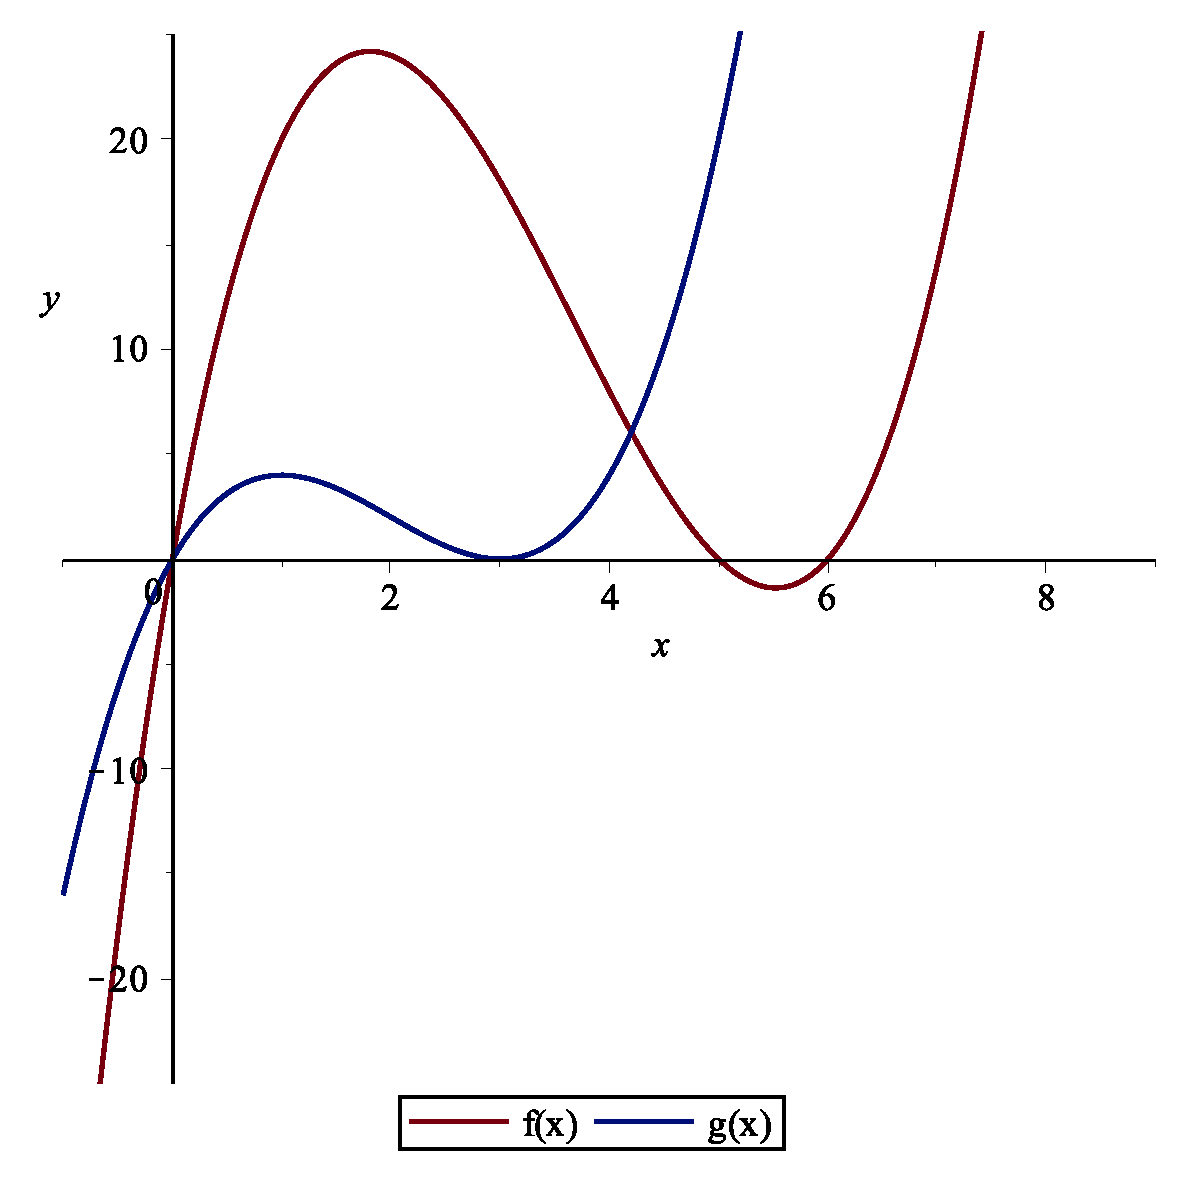
\includegraphics[scale=0.3]{images/ganzrationale_funkt_1.eps}
\end{center}
Der $G_g$ berührt bei $x=3$ die x-Achse. Wir nennen $x_{2,3}=3$ eine \underline{doppelte Nullstelle}.\\\\
Die Funktion
\begin{equation}h : \mathbb{R} \mapsto \mathbb{R} \quad \mbox{mit} \quad h(x) = (x-1)(x+3)^3\end{equation}
besitzt
\begin{itemize}
\item eine einfache Nullstelle $x_1 = 1$
\item die \underline{dreifache Nullstelle} $x_{2,3,4} = -3$\end{itemize}
\begin{center}
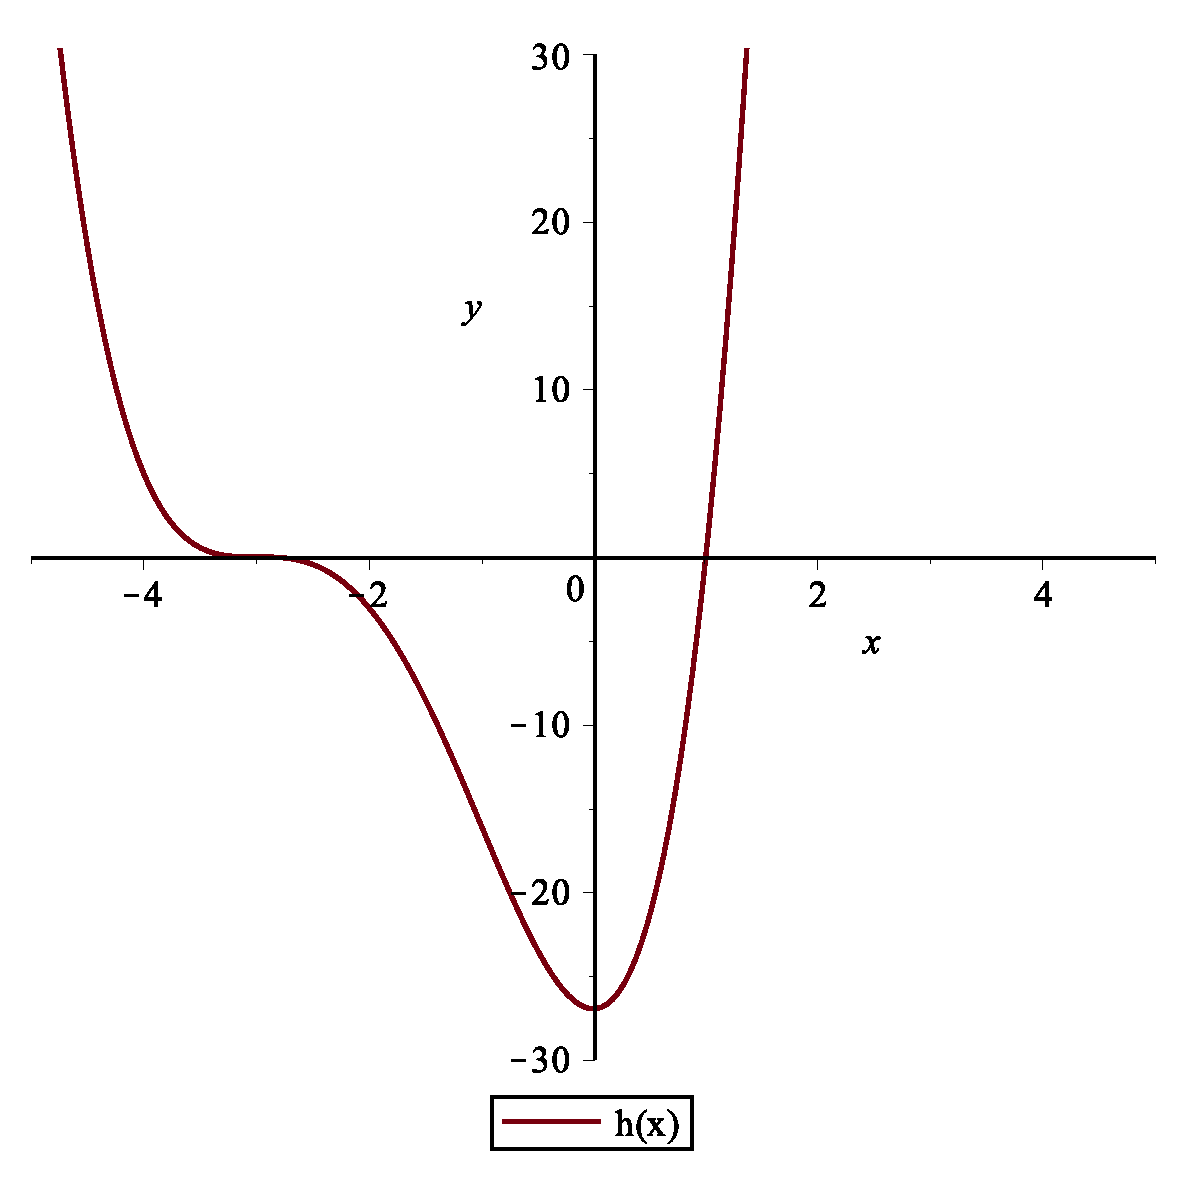
\includegraphics[scale=0.3]{images/ganzrationale_funkt_h.eps}
\end{center}
Der Graph besitzt einen \underline{Terrassenpunkt}. Ist die Nullstelle \underline{vierfach} wie bei
\begin{equation}i: \mathbb{R} \mapsto \mathbb{R} \quad \mbox{mit} \quad i(x) = (x+2)(x-3)^4\end{equation}
so besitzt der Graph einen \underline{Flachpunkt} auf der x-Achse.
\begin{center}
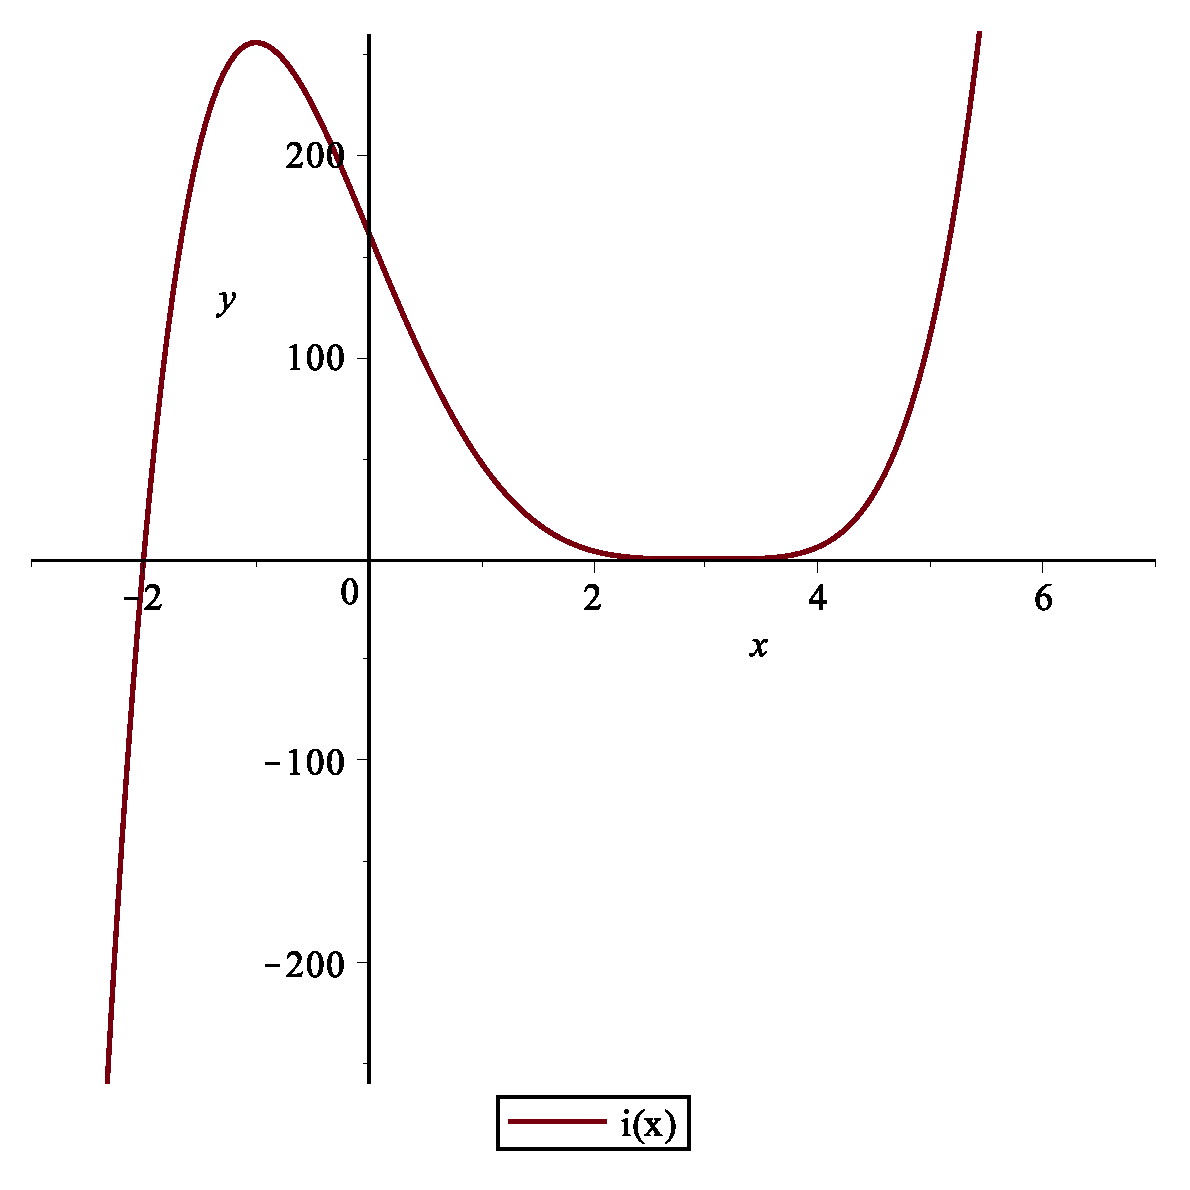
\includegraphics[scale=0.3]{images/ganzrationale_funkt_i.eps}
\end{center}
\begin{satz}Es gilt auch
\begin{equation}f(x) = x^n \to f'(x) = nx^{n-1} \quad \mbox{gilt für} \quad n \in \mathbb{Z}\end{equation}
Beweis mit vollständiger Induktion.\end{satz}
\begin{satz}Weiter ist
\begin{equation}f(x) = x^r \to f'(x) = r \cdot x^{r-1} \quad \mbox{gilt für} \quad r \in \mathbb{Q}\end{equation}
Beweis siehe Literatur.\end{satz}
\begin{myexample}\begin{eqnarray}f(x) & = & \sqrt[3]{x} + \frac{1}{\sqrt{x}} = x^{\frac{1}{3}} + x^{-\frac{1}{2}} \nonumber \\
f'(x) & = & \frac{1}{3}x^{\frac{1}{3}-1} + (-\frac{1}{2})x^{-\frac{1}{2}-1} \nonumber \\
& = & \frac{1}{3}x^{-\frac{2}{3}}-\frac{1}{2}x^{-\frac{3}{2}}\nonumber \\
& = & \frac{1}{3\sqrt[3]{x^2}} - \frac{1}{2\sqrt{x^3}} 
\end{eqnarray}\end{myexample}
\section{Höhere Ableitungen und Kurvendiskussion}
Ist $f$ eine differenzierbare Funktion und $f'$ ihre 1. Ableitung, so können wir $f'$ erneut ableiten und erhalten die \underline{2. Ableitung f''}. Fahren wir so fort, so entstehen $f''$, $f^{(4)}$, $f^{(5)}$ ... und schliesslich die \underline{n-te Ableitung $f^{(n)}$}.
\begin{myexample}\begin{equation}f: \mathbb{R} \mapsto \mathbb{R} \quad \mbox{mit} \quad f(x) = 4x^3+2x^2 -6x+10\end{equation}
\begin{eqnarray}\to f'(x) & = & 12x^2 + 4x -6 \nonumber \\
f''(x) & = & 24x + 4 \nonumber \\
f'''(x) & = & 24 \nonumber \\
f^{(4)}(x) & = & f^{(5)}(x) = f^{(n)}(x) = 0 
\end{eqnarray}\end{myexample}
Welche Informationen für $f$ erhalten wir mit $f''$?
\\\\TODO\\\\
\begin{itemize}
\item Ist $f'(x) = 0$ und $f'(x) < 0$, so besitzt $f$ ein \underline{relatives Maximum} und $G_f$ einen \underline{Hochpunkt}. (Bsp: $x_2$)
\item Ist $f'(x) = 0$und $f''(x) > 0$, so besitzt $f$ ein \underline{relatives Minimum} und $G_f$ einen \underline{Tiefpunkt}. (Bsp: $x_1, x_3$)
\item Ist $f'(x) = 0$ und $f''(x) = 0$, so besitzt $G_f$ einen \underline{Terassenpunkt}. (Bsp: $x_3$)
\item Ist $f''(x) > 0$, so ist $G_f$ \underline{konvex} oder \underline{linksgekrümmt}.
\item Ist $f''(x) < 0$, so ist $G_f$ \underline{konkav} oder \underline{rechtsgekrümmt}.
\item Ist $f''(x) = 0$, so besitzt $G_f$ einen \underline{Wendepunkt}
\end{itemize}
Bei einer \underline{Kurvendiskussion} bestimmen wir
\begin{itemize}
\item Nullstellen ($f(x) = 0$)
\item Extremwerte (mit horizontalen Tangenten ($f'(x)=0$))
\item Wendepunkte ($f''(x)=0$)
\item Graph
\end{itemize}
\begin{myexample}
\begin{enumerate}
\item TODOs
\item TODO\end{enumerate}
\end{myexample}
\section{Extremalwertprobleme}
Stellen wir uns die Frage nach dem kleinsten Benzinverbrauch, dem grössten Gewinn usw. und gelingt es uns, das Problem mit Hilfe einer Funktion zu formulieren, so können wir die Lösung mit der Differenzialrechnung finden.
\\\\TODO\\\\
Wie müssen wir Länge und Breite wählen, um mit 400m Maschendrahtzaun die grösstmögliche Fläche zu umzäunen?
\begin{enumerate}
\item \underline{Gesuchte Grösse berechnen}
\begin{equation}F = a \cdot b\end{equation}
\item \underline{Eine der auftretenden Grössen als Variable wählen}
\begin{quote}$b$ sei die Variable\end{quote}
\item \underline{Alle anderen Grössen mit Hilfe der Variablen und den bekannten Werten bestimmen}
\begin{eqnarray}a + 2b & = & 400 \nonumber \\
a & = & 400 - 2b\end{eqnarray}
\item \underline{Funktion und Definitionsmenge bestimmen}
\begin{eqnarray}F(b) & = & (400 - 2b) \cdot b\nonumber \\
& = & 400b - 2b^2\end{eqnarray}
mit
\begin{eqnarray}D_f & = & \{ b \quad | \quad 0 < b < 200 \quad \land \quad b \in \mathbb{R}\}\nonumber \\
& = & ]0;200[\end{eqnarray}
\\\\TODO: Graphs\\\\
\item \underline{Extremwerte berechnen}
\begin{equation}F'(b) = 400- 4b\end{equation}
$F'(b)$ ist $0$, wenn $b = 100$
\item \underline{Lösung diskutieren und alle gesuchten Grössen berechnen}
\\\\$b \in D_f$ und mit $F''(b) = -4$ wird $F''(100) < 0$, also ist bei $b = 100$ ein lokales Maximum.\\
Also ist $b=100, a=200$ und $F_{max} = 20000$
\end{enumerate}
Wählen wir einen Halbkreis, also ist
\begin{quote}$U = 400 = r \cdot \pi \rightarrow r = \frac{400}{\pi}$\end{quote}
und so
\begin{equation}F(Halbkreis) = \frac{r^2 \pi}{2} = \frac{\pi}{2}(\frac{400}{\pi})^2 = \frac{400^2}{2 \pi} = 25464,79\end{equation}
\begin{myproof}Beweis der Ableitung $f'(x)$: Wir beweisen mit vollständiger Induktion.
\begin{enumerate}
\item Behauptung ist für $n=1$ wahr, denn
\begin{equation}\frac{dx}{dy} = \lim_{h \to 0}\frac{(x+h)^1 - x^1}{h} = \frac{h}{h} = 1\end{equation}
und
\begin{equation}1 \cdot x^{1-1} = 1 \cdot x^0 = 1\end{equation}
\item Voraussetzung:
\begin{equation}\frac{(x+h)^n - x^n}{h} = n \cdot x^{n-1}\end{equation}
Behauptung:
\begin{eqnarray}&&\lim_{h \to 0}\frac{(x+h)^{(n+1)} - x^{(n+1)}}{h} = n \cdot x^{n-1} \nonumber \\
& = & \lim_{h \to 0}\frac{x^{n+1}h^0 + (n+1)x^nh^1 + ... + (n+1)x^1h^n + x^0h^{n+1}-x^{(n+1)}}{h} \nonumber \\
& = & \lim_{h \to 0} (n+1) \cdot x^n + ... + x^0h^n \nonumber \\
& = & (n+1)x^n\end{eqnarray}
und
\begin{equation}(n+1) \cdot x^{(n+1)-1} = (n+1) x^n\end{equation}
\item Nach (1) gilt die Behauptung für $n=1$ und nach (2) gilt sie für $n+1$, falls sie für $n$ gilt. Also gilt sie für $n = 2$ und nach (2) für $n+1$, ist 3 usw. Also gilt die Behauptung für alle $n \in \mathbb{N}$. \end{enumerate}
\qed\end{myproof}
\section{Winkelfunktionen, Produktregel}
Wir suchen die Ableitung von
\begin{equation}f: \mathbb{R} \mapsto [-1 ; 1] \quad \mbox{mit} \quad f(x) = \sin x\end{equation}
Mit
\begin{equation}f'(x) = \lim_{h \to 0}\frac{\sin(x+h) - \sin x}{h}\end{equation}
und
\begin{equation}\sin \alpha - \sin \beta = 2 \cdot \cos(\frac{\alpha + \beta}{2}) \cdot \sin(\frac{\alpha - \beta}{2})\end{equation}
wird
\begin{eqnarray}\sin(x+h) - \sin x & = & 2 \cdot \cos(\frac{x+h+x}{2}) \cdot \sin(\frac{(x+h)-x}{2}) \nonumber \\
& = & 2 \cdot \cos(\frac{2x + h}{2}) \sin(\frac{h}{2})\end{eqnarray}
und damit
\begin{eqnarray}f'(x) & = & \lim_{h \to 0} \frac{1}{h} \cdot (2\cos(\frac{2x+h}{2}) \cdot \sin(\frac{h}{2}) \nonumber \\
& = & \lim_{h \to 0} \frac{2}{h} \cdot (\cos(\frac{2x+h}{2}) \cdot \sin(\frac{h}{2}) \nonumber \\
& = & \lim_{h \to 0} \cos(\frac{2x + h}{h}) \cdot \frac{\sin(\frac{h}{2})}{\frac{h}{2}}\end{eqnarray}
Um $\lim_{h \to 0} \frac{\sin \frac{h}{2}}{\frac{h}{2}}$ zu bestimmen, betrachten wir den Sinus im Einheitskreis bei $0$.
\\\\TODO: Zeichnung\\\\
Ist $\alpha$ im Bogenmass, so ist
\begin{equation}\sin \alpha < \alpha < \tan \alpha\end{equation}
\begin{equation}\sin \alpha < \alpha < \frac{\sin \alpha}{\cos \alpha}\end{equation}
\begin{equation}1 < \frac{\alpha}{\sin \alpha} < \frac{1}{\cos \alpha}\end{equation}
\begin{equation}1 > \frac{\sin \alpha}{\alpha} > \cos \alpha\end{equation}
\begin{equation}1 \geq \lim_{\alpha \to 0} \frac{\sin \alpha}{\alpha} \geq \lim_{\alpha \to 0} \cos \alpha\end{equation}
\begin{equation}1 \geq \lim_{\alpha \to 0} \frac{\sin \alpha}{\alpha} \geq 1\end{equation}
\textcolor{red}{\begin{equation}\lim_{\alpha \to 0} \frac{\sin \alpha}{\alpha} = 1\end{equation}}
Schliesslich finden wir
\begin{eqnarray}f'(x) & = & \lim_{h \to 0} \cos \frac{2x+h}{2} \cdot \frac{\sin \frac{h}{2}}{\frac{h}{2}} \nonumber \\
& = & \cos x \cdot 1 \nonumber \\
& = & \cos x\end{eqnarray}
\textcolor{red}{\begin{equation}f(x) = \sin x \quad \to \quad f'(x) = \cos x\end{equation}}
Analog finden wir
\begin{equation}g(x) = \cos x \quad \to \quad g'(x) = -\sin x\end{equation}
\begin{myexample}\begin{enumerate}
\item \begin{eqnarray}f(x) & = & x^2 + 3 \cdot \cos x \nonumber \\
\to f'(x) & = & 2x - 3 \cdot \sin x\end{eqnarray}
\item \begin{eqnarray}\lim_{\alpha \to 0} \frac{\sin (7 \alpha)}{4 \alpha} & = & \lim_{\alpha \to 0} \frac{\frac{7}{4} \sin(7 \alpha)}{\frac{7}{4} \cdot 4 \alpha} \nonumber \\
& = & \lim_{\alpha \to 0} \frac{\frac{7}{4} \sin(7 \alpha)}{7 \alpha} \nonumber \\
& = & \frac{7}{4} \lim_{\alpha \to 0} \frac{\sin(7\alpha)}{7 \alpha} \nonumber \\
& = & \frac{7}{4} \cdot 1 = \frac{7}{4}\end{eqnarray}
\item \begin{eqnarray}\lim_{\beta \to 0} \frac{\sin(2\beta)}{cos \beta} & = & \lim_{\beta \to 0} \frac{2 \sin \beta \cos \beta}{\cos \beta} \nonumber \\
& = & \lim_{\beta \to 0} 2 \sin \beta = 0\end{eqnarray}
\end{enumerate}\end{myexample}
Um $f(x) = \sin(2x)$ ableiten zu können, formen wir zu
\begin{equation}f(x) = 2 \cdot \sin x \cos x\end{equation}
um. Wir brauchen also eine Regel, um das Produkt
\begin{equation}h'(x) = f(x) \cdot g(x)\end{equation}
zweier Funktionen ableiten zu können. Es ist
\begin{eqnarray}h'(x) & = & \lim_{h \to 0} \frac{f(x+h) \cdot g(x+h) - f(x)g(x)}{h} \nonumber \\
& = & \lim_{h \to 0} \frac{f(x+h) \cdot g(x+h) - f(x) \cdot g(x+h) + f(x)\cdot g(x+h) - f(x)g(x)}{h} \nonumber \\
& = & \lim_{h \to 0} \frac{f(x+h)g(x+h) - f(x)g(x+h)}{h} + \frac{f(x)g(x+h)-f(x)g(x)}{h} \nonumber \\
& = & \lim_{h \to 0} \frac{f(x+h)-f(x)}{h} g(x+h)+f(x) \cdot \frac{g(x+h)-g(x)}{h} \nonumber \\
& = & f'(x) \cdot g(x) + f(x) \cdot g'(x)\end{eqnarray}
Damit finden wir die Produktregel:
\textcolor{red}{\begin{equation}(fg)' = f'g + fg'\end{equation}}
\begin{myexample}Berechne die Ableitung von
\begin{enumerate}
\item \begin{eqnarray}f(x) & = & x^2 \cdot \cos(x) \\
u(x) & = & x^2 \\
v(x) & = & \cos(x)\end{eqnarray}
Mit
\begin{eqnarray}u'(x) & = & 2x \nonumber \\
v'(x) & = & -\sin(x)\end{eqnarray}
finden wir
\begin{eqnarray}f'(x) & = & 2x \cdot \cos(x) + x^2 \cdot (-\sin(x)) \nonumber \\
& = & 2x \cdot \cos(x) - x^2 \cdot \sin(x)\end{eqnarray}
\item \begin{eqnarray}g(x) & = & \sin(2x) = 2 \sin(x) \cos(x) \nonumber \\
& = & 2(\cos^2(x) - \sin^2(x)) \nonumber \\
& = & 2 \cos(2x)\end{eqnarray}
\end{enumerate}
Wir werden zeigen, dass
\begin{equation}(\sin(k \cdot x))' = k \cdot \cos(k \cdot x), \quad k \in \mathbb{R}\end{equation}
Es wird also
\begin{eqnarray}h(x) & = & \cos(2x) = \cos^2(x) - \sin^2(x) \nonumber \\
& = & 1 - 2 \sin^2(x)\end{eqnarray}
und mit
\begin{equation}i(x) = \sin^2(x) = \sin(x) \cdot \sin(x)\end{equation}
wird
\begin{eqnarray}i'(x) & = & \sin(x) \cdot \cos(x) + \sin(x) \cdot \cos(x) \nonumber \\
& = & 2 \sin(x) \cdot \cos(x) \nonumber \\
& = & \sin(2x)\end{eqnarray}
Damit erhalten wir
\begin{equation}h'(x) = -2 \sin(2x)\end{equation}
Diskutiere die Funktion
\begin{equation}f: [0; 2 \pi ] \mapsto \mathbb{R} \quad \mbox{mit} \quad f(x) = 2 \sin(x) + \sin(2x)\end{equation}
TODO: Exmaple fertig
\end{myexample}

\chapter{Integralrechnung}
\section{Stammfunktion}
Wir kennen die Abbildung $f'$ einer differenzierbaren Funktion $f$ und suchen $f(x)$.\\
Ist
\begin{equation}f'(x) = x^3 - x^2 + x + 4\end{equation}
so wird
\begin{equation}f(x) = \frac{x^4}{4} - \frac{x^3}{3} + \frac{x^2}{2} + 4x\end{equation}
Ist $g'(x) = \cos(x)$, so ist $g(x) = \sin(x)$. Aber auch
\begin{equation}f(x) = \frac{x^4}{4} - \frac{x^3}{3} + \frac{x^2}{2} + 4x + 11\end{equation}
\begin{equation}f(x) = \frac{x^4}{4} - \frac{x^3}{3} + \frac{x^2}{2} + 4x + \sqrt{17}\end{equation}
und
\begin{equation}g(x) = \sin(x) + 9\end{equation}
\begin{equation}g(x) = \sin(x) - \frac{7}{11}\end{equation}
\begin{mydef}Ist $f(x)$ die Ableitung einer Funktion $F(x)$, so heisst $F$ eine \underline{Stammfunktion} von $f$:
\begin{equation}F'(x) = f(x)\end{equation}
Die Menge aller Stammfunktionen heisst \underline{unbestimmtes Integral}, wofür wir
\begin{equation}\int \! f(x) \, \mathrm{d} x = F(x) + C\end{equation}
schreiben. Dabei heisst
\begin{itemize}
\item $f(x)$ der \underline{Integrand}
\item $\mathrm{d}x$ das \underline{Differential}
\item $C \in \mathbb{R}$ die \underline{Integrationskonstante}
\end{itemize}
\end{mydef}
\begin{myexample}
\begin{enumerate}Wir berechnen die unbestimmten Integrale:
\item \begin{equation}\int \! 4x^3 - 3x \, \mathrm{d} x = x^4 - \frac{3x^2}{2} + C\end{equation}
\item \begin{equation}\int \! 2 \cos(x) + 3 \sin(x) \, \mathrm{d} x = 2 \sin(x) - 3\cos(x) + C\end{equation}
\item \begin{equation}\int \! at^2 + bt + c \, \mathrm{d} t = a \frac{t^3}{3} + b \frac{t^2}{2} + ct + D\end{equation}
\begin{equation}\int \! at^2 + bt + c \, \mathrm{d} a = \frac{a^2}{2} \cdot \frac{t^2}{2} + bta + ca + D\end{equation}
\end{enumerate}\end{myexample}
Die Regeln der Differenzialrechnung übertragen sich auf die Integralrechnung
\begin{enumerate}
\item \begin{equation}\int \! f(x) + g(x) \, \mathrm{d} x = \int \! f(x) \, \mathrm{d} x + \int \! g(x) \, \mathrm{d} x\end{equation}
\item \begin{equation}k \in \mathbb{R}: \int \! k \cdot f(x) \, \mathrm{d} x = k \cdot \int \! f(x) \, \mathrm{d} x\end{equation}
\item \begin{equation}\int \! x^p \, \mathrm{d} x = \frac{x^{p+1}}{p+1} \quad ; \quad p \in \mathbb{R} \setminus \{-1\}\end{equation}
\end{enumerate}
\begin{myexample}TODO: Beispiel\end{myexample}
\section{Flächeninhalte}
Welchen Inhalt besitzt die durch den Graphen von
\begin{equation}f: \mathbb{R} \mapsto \mathbb{R}_0^+ \quad \mbox{mit} \quad f(x) = x^2\end{equation}
die Gerade $x=b$ $(b > 0)$ und die x-Achse begrenzte Fläche?
\\\\TODO: Grafik\\\\
Wir machen eine Näherung mit $n$ Rechtecken der Breite $\frac{b}{n}$, und zwar solche die "zu gross" sind mit Flächeninhalt $F_i (i=1,2,3,...,n)$ und solche, die "zu klein" sind mit Flächeninhalt $f_k (k=1,2,3,...,n)$ um den gesamten Flächeninhalt $F$ von oben und unten zu nähern.
\\\\TODO: Grafik\\\\
mit
\begin{equation}s_n = \sum_{i=1}^n F_i \quad , \quad s_n = \sum_{k=1}^n f_k\end{equation}
Es ist
\begin{equation}F_1 = \frac{b}{n} \cdot f(\frac{b}{n}) = \frac{b}{n} (\frac{b}{n})^2 = \frac{b^3}{n^3}\end{equation}•
\end{document}